Ausflug: Bluescreen Berechnung wie in Starwars mit Listen:\\

\begin{mdframed}
\begin{lstlisting}
(define yoda @
\includegraphics[scale=0.5]{Yoda}@)
(define dagobah @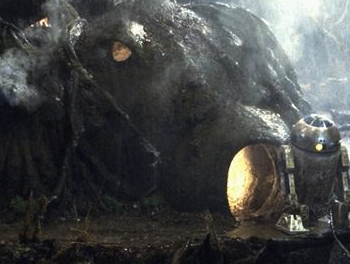
\includegraphics[scale =0.5]{dagobah}@)
;_________________________________________
;Zugriff auf die Liste der Bildpunkte (Pixel) eines Bildes: 
 
;(: image->color-list (image -> (list-of rgb-color)))  
;(: color-list->bitmap ((list-of rgb-color) natural natural -> image))
 
;Breite/Höhe eines Bildes in Pixeln:
 
;(: image-width (image -> natural))
; (: image-height (image -> natural))
 
; Eine Farbe (rgb-color) besteht aus ihrem
; - Rot-Anteil 0..255 (red)
; - Grün-Anteil 0..255 (green)
; - Blau-Anteil 0..255 (blue)

 @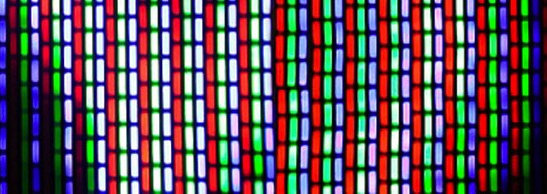
\includegraphics[scale=0.5]{pixel}@
 
; (define-record-procedures rgb-color
;   make-color
;   color?
;   (color-red color-green color-blue))
;________________________________________

; Signatur für color-Records nicht in image2.rkt eingebaut.  Roll our own...
(define rgb-color
  (signature (predicate color?)))


; Ist Farbe c bläulich?
(: bluish? (rgb-color -> boolean))
(define bluish?
  (lambda (c)
    (< (/ (+ (color-red c) (color-green c) (color-blue c))
          3)
       (color-blue c))))

; Worker:
; Pixel aus Hintergrund bg scheint durch, wenn der
; entsprechende Pixel im Vordergrund fg bläulich ist.
; Arbeite die Pixellisten von fg und bg synchron ab
; Annahme: fg und bg haben identische Länge!
(: bluescreen ((list-of rgb-color) (list-of rgb-color) -> (list-of rgb-color)))
(define bluescreen
  (lambda (fg bg)
    (cond ((empty? fg)
           empty)
          ((pair? fg)
           (make-pair 
            (if (bluish? (first fg))
                (first bg)
                (first fg))
            (bluescreen (rest fg) (rest bg)))))))

; Wrapper:
; Mische Vordergrund fg und Hintergrund bg nach Bluescreen-Verfahren
(: mix (image image -> image))
(define mix
  (lambda (fg bg)
    (let ((fg-h (image-height fg))
          (fg-w (image-width fg))
          (bg-h (image-height bg))
          (bg-w (image-width bg)))
      (if (and (= fg-h bg-h)
               (= fg-w bg-w))
          (color-list->bitmap
           (bluescreen (image->color-list fg)
                       (image->color-list bg))
           fg-w
           fg-h)
          (violation "Dimensionen von Vorder-/Hintergrund verschieden")))))

; Yoda vor seine Hüte auf Dagobah setzen
(mix yoda dagobah) @\eval \ 
\includegraphics[scale=0.5]{Yoda_finished}@
\end{lstlisting}
\end{mdframed}\ \\

Generierung aller natürlichen Zahlen (vgl. gemischte Daten)\\
Eine natürliche Zahl (natural) ist entweder 
\begin{enumerate}[-]
\i die 0 (zero)
\i der Nachfolge (succ) einer natürlichen Zahl
\end{enumerate}

$\mathbb{N} = \{0, (succ(0)), (succ(succ(0))), \ldots \} $\\
\uline{Konstruktoren}\\
\begin{lstlisting}
(: zero natural)
(define zero 0)
(: succ (natural -> natural))
(define succ (lambda (n)(+ n 1)))
\end{lstlisting}
Vorgänger (pred), definiert für $n > 0$
\begin{lstlisting}
(: pred (natural -> natural))
(define pred
	(lambda (n) (- n 1)))
\end{lstlisting}
Bedingte algebraische Eigenschaft (für check-property):\\
\code{(==\zu \ \auf p\zu \argt{})}\\
Nur wenn \auf p \zu \eval \# t ist, wird Ausdruck \argt{} ausgwertet und getestet \argt{} \eval \# t
\begin{lstlisting}[frame =single]
; Eigenschaft nur auswerten, wenn n > 0 (==>)
(check-property
 (for-all ((n natural))
   (==> (> n 0)   
        (= (succ (pred n)) n))))
\end{lstlisting}

Beispiel für Rekursion auf natürlichen Zahlen: Fakultät\\$
\begin{array}{rcl}
0! &=& 1\\
n! &=& n \cdot (n -1)!\\
&\\
3! &=& 3 \cdot 2!\\
&=& 3 \cdot 2 \cdot 1!\\
&=& 3 \cdot 2 \cdot 1 \cdot 0!\\
&=& 3 \cdot 2 \cdot 1 \cdot 1\\
&=& 6\\
&\\
10 &=& 3628800
\end{array}$\bigskip \\
\begin{lstlisting}[frame =single]
; Berechne n!
(: factorial (natural -> natural))
(check-expect (factorial 0) 1)
(check-expect (factorial 3) 6)
(check-expect (factorial 10) 3628800)

(define factorial
  (lambda (n)
    (cond ((= n 0) 1)
          ((> n 0) (* n (factorial (- n 1)))))))
\end{lstlisting}
Konstruktionsanleitung für Prozeduren über natürlichen Zahlen:\\
\begin{lstlisting}
(:<f> (natural -> <t>))
	(define <f>
		(lambda (n)
			(cond ((= n 0)...)
				((> n 0) ... (<f> (- n 1))...))))
\end{lstlisting}
Beobachtung:\\
\begin{enumerate}[-]
\i Im letzten Zweig ist $n > 0 \rightarrow$ pred angewandt
\i \code{(\argf{} (- n 1))} hat die Signatur \argt{}
\end{enumerate}
Satz:\\
Eine Prozedur, die nach der Konstruktionsanleitung für Listen oder natürliche Zahlen konstruiert wurde \uline{terminiert immer} (= liefert immer ein Ergebnis).\\
(Beweis in Kürze)\\
\begin{lstlisting}[frame=single]
; Fehlerhaft: kein Fortschritt im rekursiven Aufruf
; => potentiell "unendliche" Reduktion
(define unfactorial
  (lambda (n)
    (cond ((= n 0) 1)
          ((> n 0) (* n (unfactorial n))))))

; Fehlerhaft: kein definierter Abbruch der Rekursion
; => Abbruch der Reduktion bei n = 0 ("cond: alle Tests ergaben #f")
(define not-factorial
  (lambda (n)
    (cond ((> n 0) (* n (not-factorial (- n 1)))))))
\end{lstlisting}
$\overbrace{(3 \cdot (2 \cdot (1}^{\t{merken}} \cdot 0!)))$\\
Die Grö\ss e eines Ausdrucks ist proportional zum Platzverbrauch des Reduktionsprozesses im Rechner\\
$\Rightarrow$ Wenn möglich Reduktionsprozesse, die \uline{konstanten} Platzverbrauch - unabhängig von Eingabeparametern - benötigen